{\usebackgroundtemplate{\includegraphics[height=\paperheight]{../images/zippy/bugs/buggybugs-1.jpg}}
\begin{frame}[t,plain]
    \titlepage
\end{frame}
}

\begin{frame}[fragile]
  {CTF: Capture The Flag}

  \begin{itemize}
    \item Collaborative hacking competitions
    \begin{itemize}
    	\item Teams vs. Teams
    \end{itemize}
    \item The goal is to capture flags
    \begin{itemize}
    	\item By finding and exploiting bugs
    	\item By understanding systems
    	\item By uncovering hidden secrets
    	\item By breaking crypto
    \end{itemize}
  \end{itemize}
\end{frame}

\begin{frame}[fragile,plain]
	\begin{center}
		\Huge\verb+CTF{THIS_IS_A_FLAG}+
	\end{center}
\end{frame}


\begin{frame}
  {CTF Type: Jeopardy}

  \begin{figure}[h]
    \centering
    %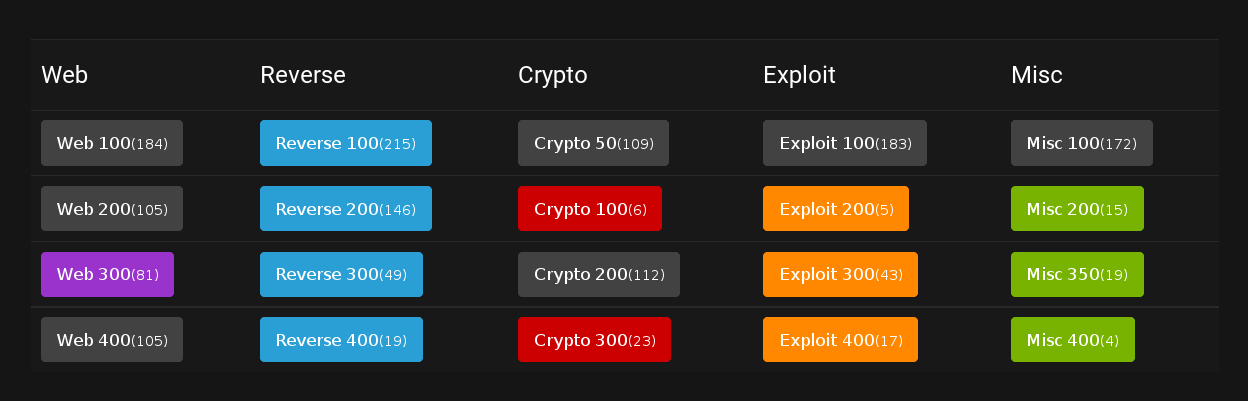
\includegraphics[width=\textwidth]{../images/dctf-challenges.png}
    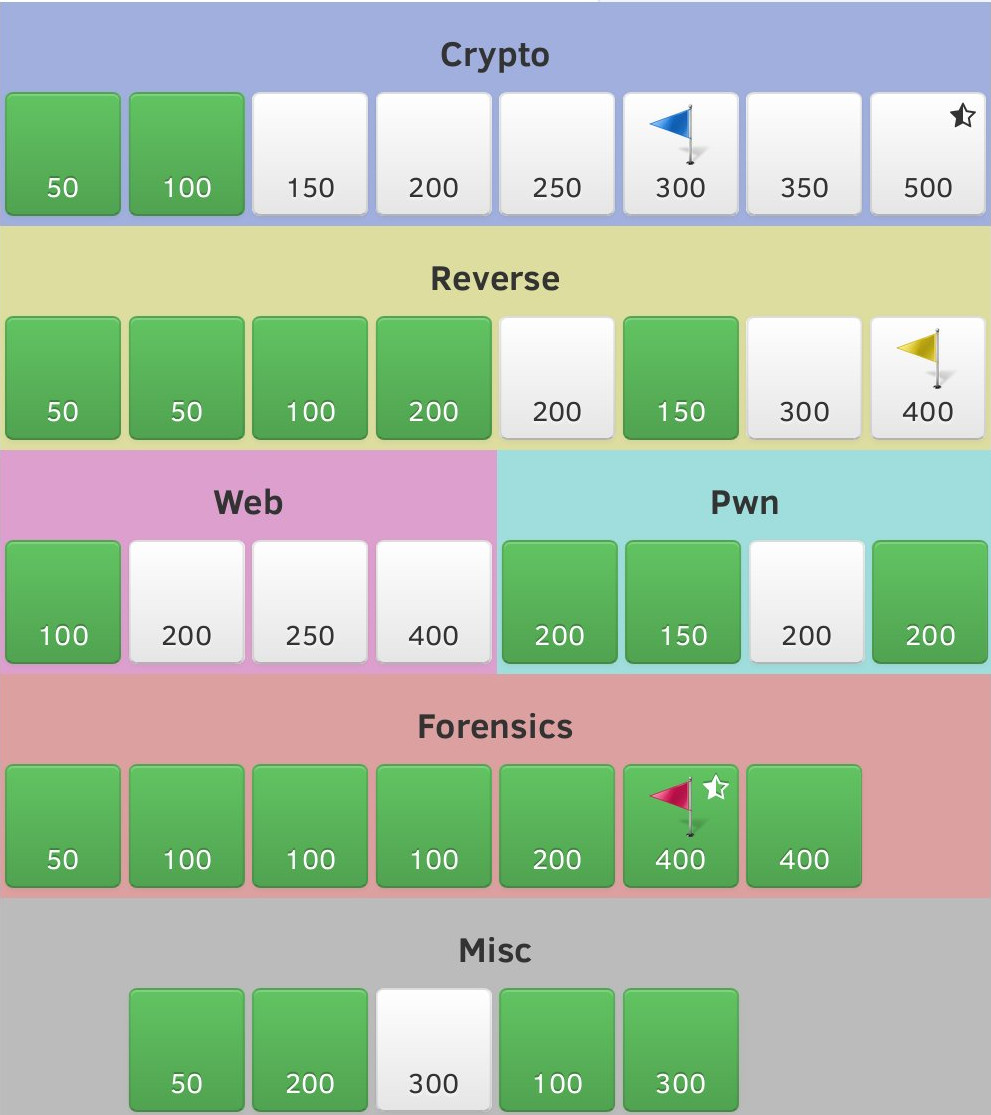
\includegraphics[height=0.8\textheight]{../images/sharifctf-challenges.jpg}
    \caption{\footnotesize{}Sharif CTF Challenge Board}
    \label{fig:jeopardyboard}
  \end{figure}
\end{frame}

\begin{frame}
  {CTF Type: Attack-Defense}

  \begin{figure}[h]
    \centering
    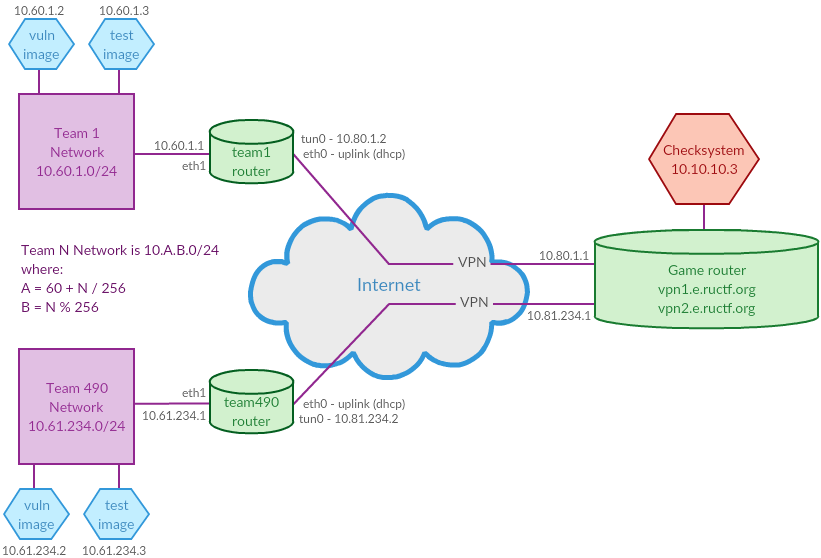
\includegraphics[width=0.9\textwidth]{../images/ructf-network.png}
    \caption{\footnotesize
      RUCTFe 2015 Network Schema (source:
      \href{https://ructf.org/e/2015/network.html}{RUCTF org}) }
  \end{figure}
\end{frame}

\begin{frame}
  {CTF Type: Attack-Defense}

  \begin{figure}[h]
    \centering
    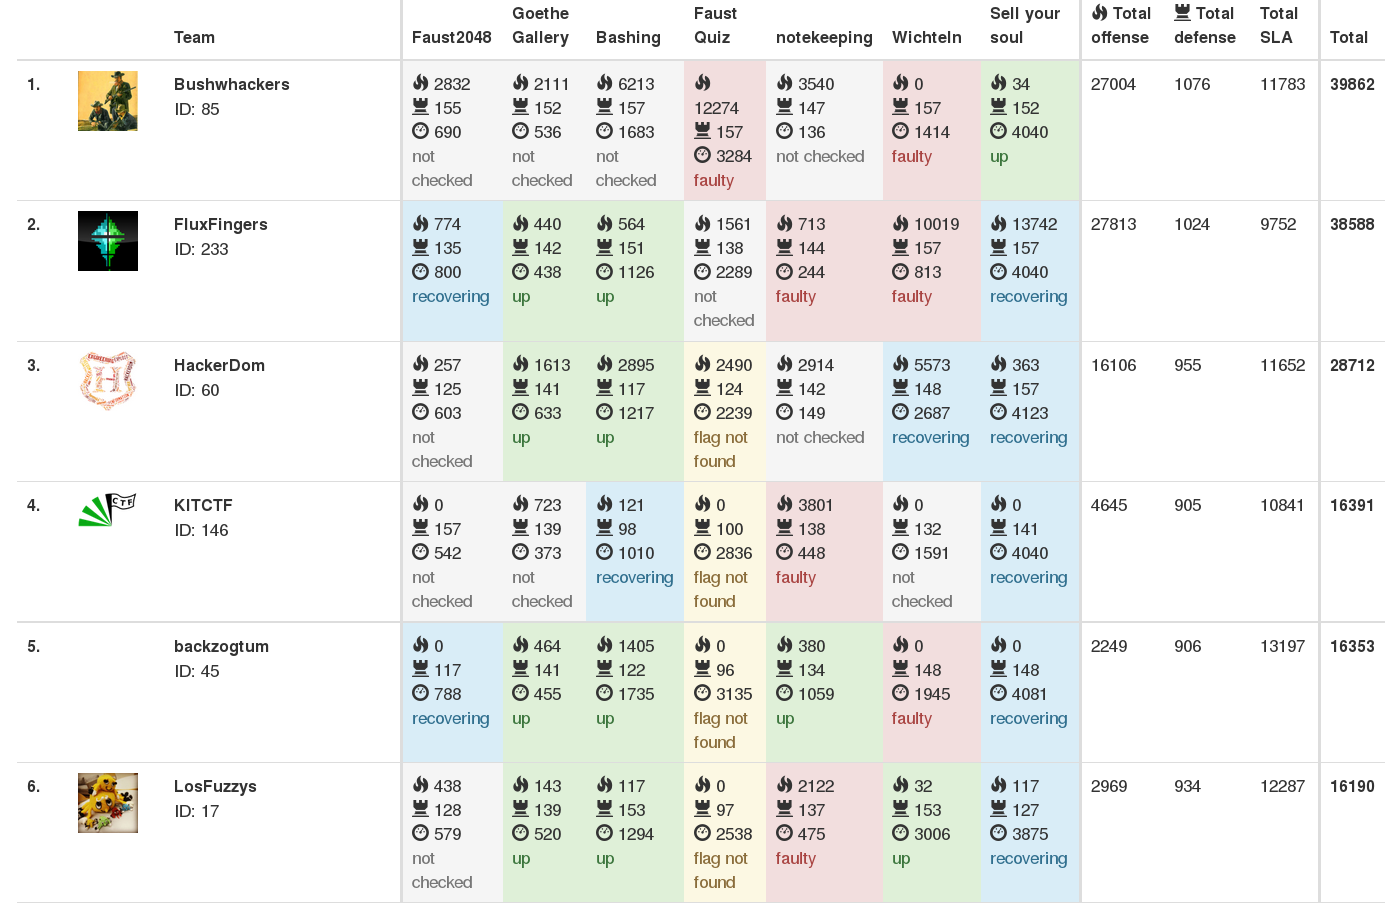
\includegraphics[width=\textwidth]{../images/faustctf-scoreboard.png}
    \caption{\footnotesize{}FAUST CTF 2015 scoreboard}
    \label{fig:faustctfscoreboard}
  \end{figure}

\end{frame}


\begin{frame}
  {Why CTFs?}

  \begin{itemize}
    \item \textbf{It's fun!}
    \item Gain experience in Information Security
    \item Challenges modeled after real-world problems
      \begin{itemize}
        \item Sometimes real-world bugs modeled after CTF bugs?
      \end{itemize}
  \end{itemize}
\end{frame}


{\usebackgroundtemplate{\includegraphics[height=\paperheight]{../images/zippy/bugs/buggybugs-20.jpg}}
\begin{frame}[allowframebreaks,plain]

  {\huge
    \texttt{LosFuzzys}: A CTF Team in Graz}

  \vspace{19em}

  {\Large
  We Like Bugs!}

\end{frame}
}

\begin{frame}
  {LosFuzzys: A CTF Team in Graz}

  \begin{itemize}
    \item A group of people interested in information security
    \item Primarily CS/SW/ICE Students from TUGraz
      \begin{itemize}
        \item We welcome anyone interested and motivated
        \item so maybe you :)
      \end{itemize}
    \item Current \href{https://ctftime.org/team/8323}{ctftime.org} ranking
      (2016-11-23)
      \begin{itemize}
        \item Global place 49 (of about 9000 teams)
        \item 2nd place in Austria
      \end{itemize}
    \item Regular Meet-ups/Trainings: Wednesday 18:15 @ IAIK
      \begin{itemize}
        \item Next training session: 7. December
        \item Announced on mailing list and calendar
      \end{itemize}
  \end{itemize}
\end{frame}


\begin{frame}[plain]

  \vspace{12em}

  \begin{columns}[T]
    \begin{column}{.6\textwidth}
      \begin{rotate}{-5}
        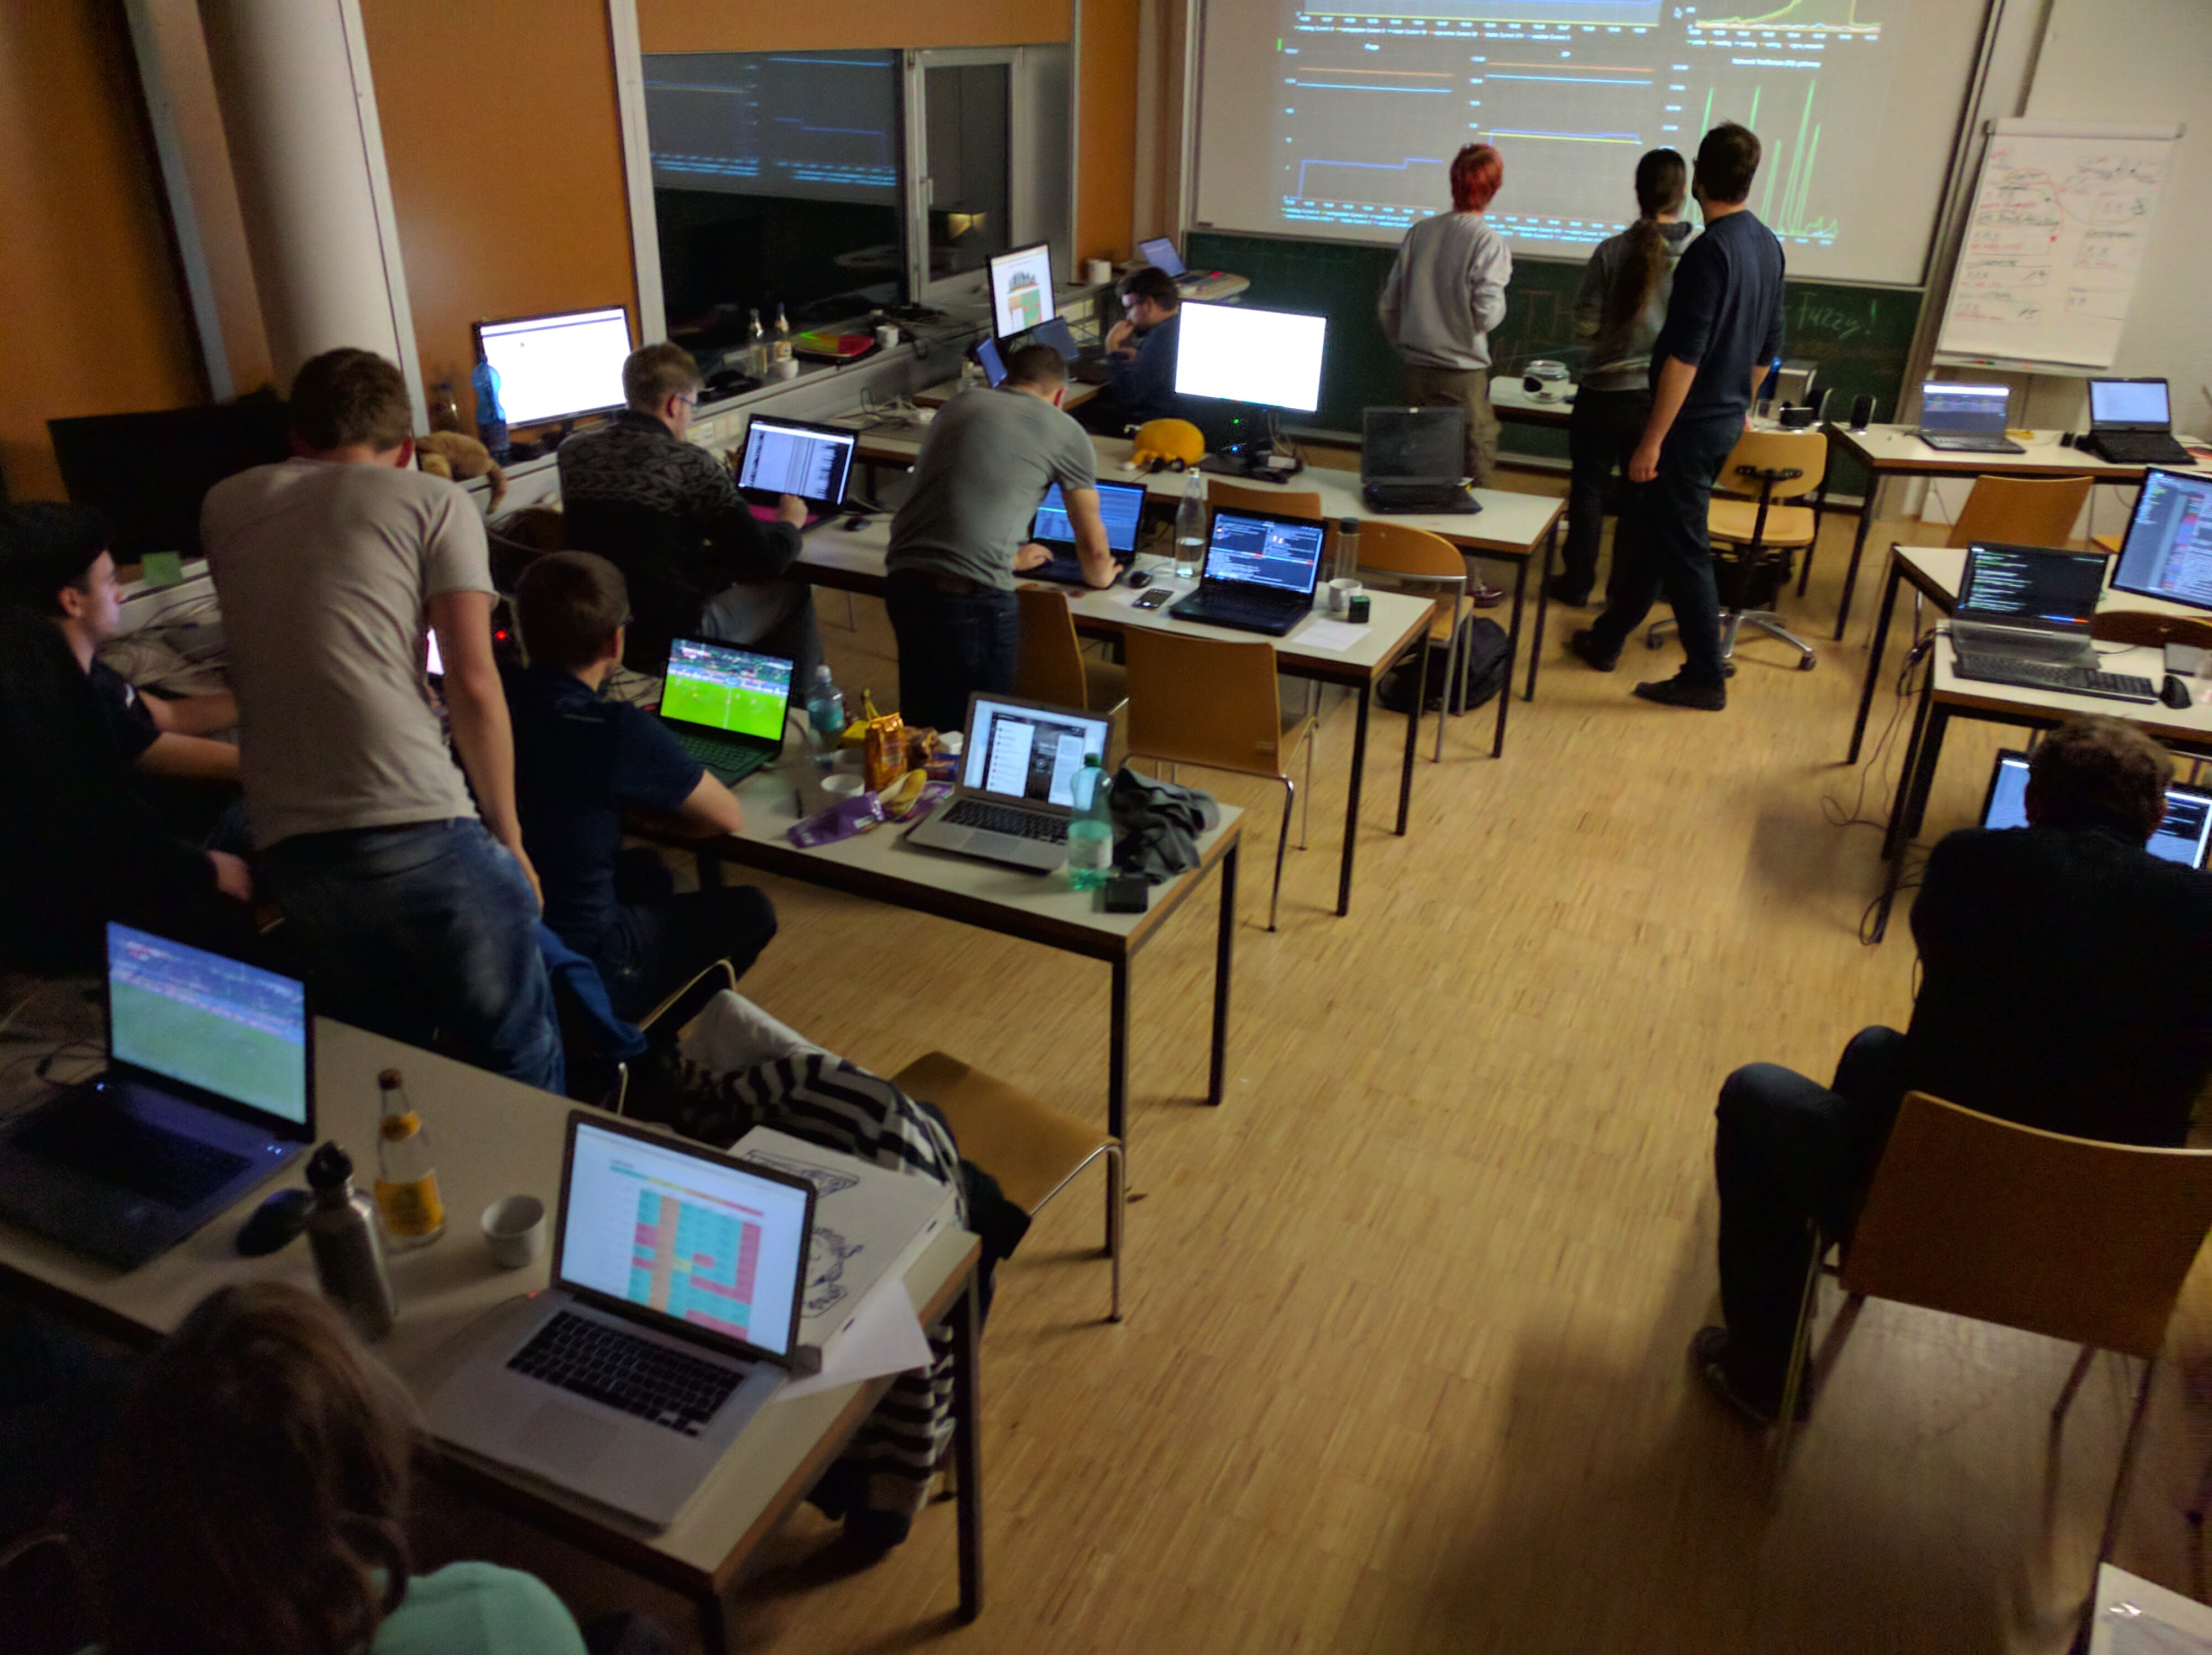
\includegraphics[width=\textwidth]{../images/ructfe2016-hacking.jpg}
      \end{rotate}
    \end{column}
    \begin{column}{.4\textwidth}
      \begin{rotate}{5}
        \includegraphics[width=\textwidth]{../images/r2-training-session.jpg}
      \end{rotate}

      \vspace{7em}

      \begin{rotate}{-7}
        \includegraphics[width=\textwidth]{../images/pwn-training-session.jpg}
      \end{rotate}
    \end{column}
  \end{columns}
\end{frame}

\begin{frame}[fragile]
	{Where to start?}

	\begin{itemize}
    \item Talk to us! :-)
      \begin{itemize}
        \item During Bachelor @ IAIK on 2. December
        \item During our training sessions Wednesdays 18:15 @ IAIK
      \end{itemize}
  \end{itemize}

  \begin{columns}[T]
    \begin{column}{.55\textwidth}
      \begin{itemize}
        \item \url{https://hack.more.systems}
        \item Mail: \href{mailto:we@hack.more.systems}{we@hack.more.systems}
        \item Twitter: \href{https://twitter.com/LosFuzzys}{@LosFuzzys}
        \item Subscribe to our mailing list  % with your \texttt{student.tugraz.at} mail \(\rightarrow\)
      \end{itemize}

    \end{column}

    \begin{column}{.45\textwidth}
      %\begin{center}
        %\qrcode[hyperlink,height=0.9\textwidth]{https://mail.htu.tugraz.at/cgi-bin/mailman/listinfo/losfuzzys}
        \qrcode[hyperlink,height=0.95\textwidth]{https://hack.more.systems}
      %\end{center}
    \end{column}
  \end{columns}

\end{frame}


